\documentclass{exam}

\usepackage{units} 
\usepackage{graphicx}
\usepackage[fleqn]{amsmath}
\usepackage{cancel}
\usepackage{float}
\usepackage{mdwlist}
\usepackage{booktabs}
\usepackage{cancel}
\usepackage{polynom}
\usepackage{caption}
\usepackage{fullpage}
\usepackage{xfrac}
\usepackage{enumerate}

\newcommand{\degree}{\ensuremath{^\circ}} 
\everymath{\displaystyle}

\printanswers

% \begin{figure}[H]
%   \centering
%   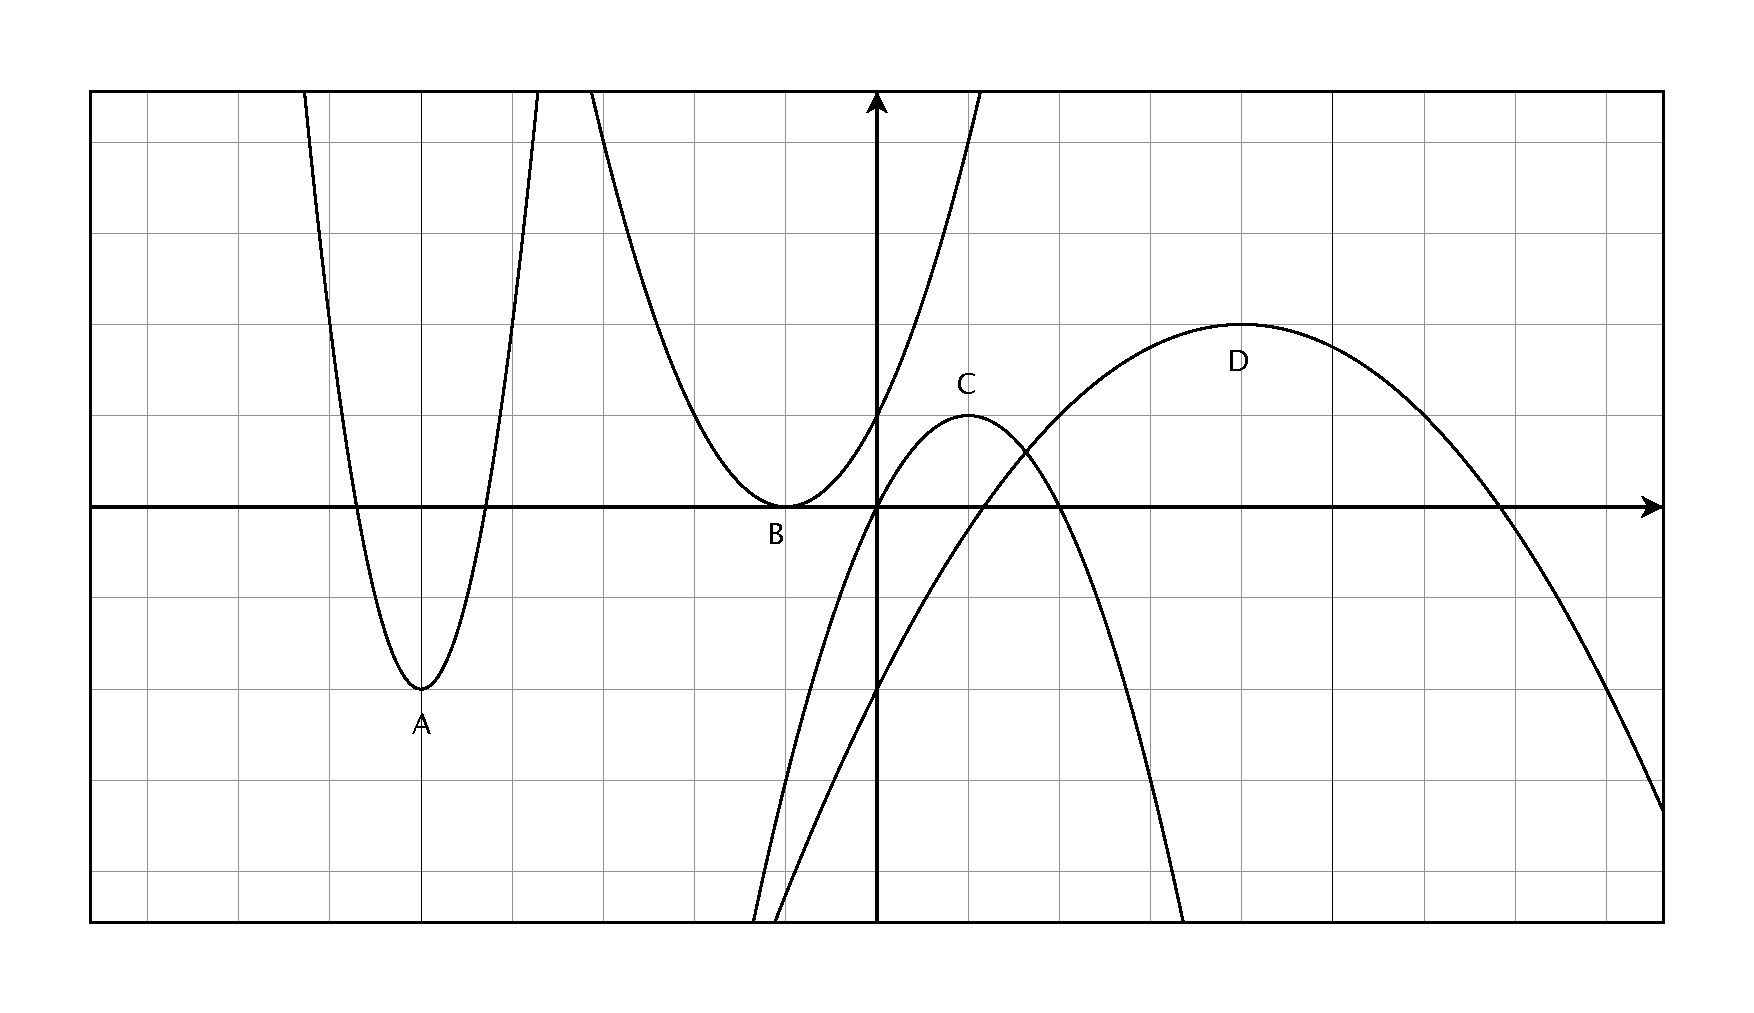
\includegraphics[scale=.3]{problem_7.eps}
%   \caption*{Problem 7}
% \end{figure}

% \begin{tabular}{cc}
% \toprule
% period & amplitude \\
% \midrule
%   $\pi$ & $2$ \\
% \bottomrule
% \end{tabular}

\title{Math 141 Notes \\ Section 4.5}

\date{July 3, 2013}

\begin{document}

  \maketitle
  \tableofcontents

  \section{Homework}
  \begin{enumerate}
    \item
      \[
        \ln 3x^2 = \ln 3 + 2 \ln x \neq 2 \left( \ln 3 + \ln x \right)
      \]
      Only $x$ is squared.

    \item $\log_a a = 1$

  \end{enumerate}

  \section{Population Growth}

  \subsection{Description}
  Just like compound interest: $n(t) = n_0 e^{rt}$.

  \begin{itemize*}
    \item $n$ population at time $t$
    \item $n_0$ initial population
    \item $r$ growth rate--the percentage of the population that produces a new instance each interval
    \item $t$ time
  \end{itemize*}

  \subsection{Examples}

  \begin{enumerate}
    \item bacteria with:
      \begin{itemize*}
        \item $n_0 = 1,000$ 
        \item $r = \unit[0.3]{hr}$; 30\% divide each hour
      \end{itemize*}

      \begin{enumerate}[a]
        \item find the function 
          \[
            n(t) = 1,000 e^{0.3 t}
          \]

        \item how many bacteria after 5 hours? 
          \[
            n(5) = 1,000 e^{0.3 \cdot 5} \approx 4,482
          \]

        \item how many bacteria after 24 hours? 
          \[
            n(24) = 1,000 e^{0.3 \cdot 24} \approx 1,339,430
          \]

        \item how many bacteria were present 2 hours ago? 
          \begin{align*}
            1,000 & = n_0 e^{.3 \cdot 2} \\
            n_0   & \approx 549
          \end{align*}

        \item when did the experiment start with 1 bacterium?
          \begin{align*}
            1,000 & = e^{.3 \cdot t} \\
            t     & \approx \unit[23]{hr}
          \end{align*}

        \item another species propagates at a different rate and reaches 1,000 bacteria in just 8 hours.  What is the
          rate for this species?
          \begin{align*}
            1,000 & = e^{r \cdot 8} \\
            r     & \approx 0.691
          \end{align*}

      \end{enumerate}

    \item 2,000 bacteria; the population doubles every 3 hours
      
      \begin{enumerate}[a]
        \item find the rate:
          \begin{align*}
            2n_0 & = n_0 e^{3r} \\
            r    & = \frac{\ln 2}{3} \\
                 & \approx 0.231 \\
          \end{align*}

        \item how many after 2 hours?
          \[
            n(1) = 2,000 e^{0.231 \cdot 2} \approx 3,175
          \]

        \item when will there be 20,000?
          \begin{align*}
            20,000 & = 2,000 e^{0.231 t} \\
            t      & \approx \unit[9.97]{hr} \\
          \end{align*}

      \end{enumerate}
      
  \end{enumerate}

  \section{Radioactive Decay}

  \subsection{Description}
  Like growth, but with time running backwards: 
  \[
    n(t) = n_0 e^{-rt}
  \]

  \begin{itemize*}
    \item $m$ quantity at time $t$
    \item $m_0$ initial quantity
    \item $r$ decay rate
    \item $t$ time
  \end{itemize*}

  \subsection{Examples}

  \begin{enumerate}
    \item What is the rate if the half life is $T$ years?
      \begin{align*}
        \frac{m_0}{2} &= m_0 e^{-rT} \\
        -rT           &= \ln \frac{1}{2} \\
        rT            &= \ln 2 \\
        r             &= \frac{\ln 2}{T} \\
      \end{align*}

    \item What is the rate if the half life is 2,000 years?
      \[
        r = \frac{\ln 2}{2,000} \approx 0.000346574 \\
      \]

    \item How old is a sample if 35\% remains and the half life is 2,000 years?
      \begin{align*}
        0.35 m_0 & = m_0 e^{0.000346574 t} \\
        t        & \approx \unit[3,029]{yr} \\
      \end{align*}

    \item How much of an original sample of 100 kg remains after 10,000 years?
      \begin{align*}
        m & = 100 e^{0.000346574 \cdot 10,000} \\
          & \approx \unit[3.125]{kg} \\
      \end{align*}
  \end{enumerate}

  \section{Newton's Law of Cooling}

  \subsection{Description}
  \[
    T(t) = T_s + D_0 e^{-kt}
  \]

  \begin{itemize*}
    \item $T_s$ temperature of surroundings
    \item $D_s$ initial temperature difference
    \item $k$ constant that depends on the object
    \item $t$ time
  \end{itemize*}

  \subsection{Example}
    If it's $130 \degree$ in Death Valley and an object brought from outside into an air-condition room at $70
    \degree$ cools to $110 \degree$ in 10 minutes, when will it be $80 \degree$?

    First find $k$:
    \begin{align*}
      D_0 & = 130 - 70 \\
          & = 60 \\
      \\
      110 & = 70 + 60 e^{-k \cdot 10} \\
      k   & \approx 0.0405465 \\
    \end{align*}

    Then find out when it will be $80 \degree$:
    \begin{align*}
      80 & = 70 + 60 e^{-0.0405465 t} \\
      t  & \approx \unit[44]{minute} \\
    \end{align*}

  \section{Logarithmic Scales}

  \subsection{pH}
  \subsubsection{Description}
  The log of the concentration of Hydrogen ions.
  \[
    pH = - \log(H+)
  \]

  \begin{itemize*}
    \item $H+$ concentration of hydrogen ions in moles per liter
    \item 7 is neutral
  \end{itemize*}

  \subsubsection{Examples}

  \begin{enumerate}
    \item What is the pH if the concentration is $\unit[3 \cdot 10^{-3}]{mole/liter}$?
      \[
        pH = - \log \left( 3 \cdot 10^{-3} \right) \approx 2.5
      \]

    \item What is the concentration of hydrogen ions if the pH is 3?
      \begin{align*}
        3 &= - \log H \\
        H &\approx \unit[7.9 \cdot 10^{-3}]{mole/liter}
      \end{align*}

  \end{enumerate}

  \subsection{Richter Scale}
  \subsubsection{Description}
  The Richter scale is the log of the ratio of an earthquake to the smallest measurable earthquake.
  \[
    M = \log \frac{I}{S}
  \]

  \begin{itemize*}
    \item $I$ intensity of quake 
    \item $S$ intensity of minimum measurable quake
    \item $M$ magnitude of quake on the Richter scale
  \end{itemize*}

  \subsubsection{Examples}
  \begin{enumerate}

    \item What is the intensity of a 9.5 earthquake?
      \begin{align*}
        9.5 & = \log \frac{I}{10^{-4}} \\
        I   & \approx 316,228 \\
      \end{align*}

    \item What is the magnitude of a quake with intensity 50,000?
      \begin{align*}
        M & = \log \frac{50,000}{10^{-4}} \\
           & \approx 8.7 \\
      \end{align*}

  \end{enumerate}

  \subsection{Decibels}

  \subsubsection{Description}
  Measure of loudness
  \[
    B = 10 \log \frac{I}{I_0}
  \]
  
  $I_0 = \unit[10^{-12}]{W/m^2}$--just barely audible sound 

  \begin{itemize*}
    \item $I$ intensity of sound 
    \item $I_0$ intensity of barely audible sound $I_0 = \unit[10^{-12}]{W/m^2}$
    \item $B$ magnitude of sound in decibels
  \end{itemize*}

  \subsubsection{Examples}
  \begin{enumerate}

    \item What is the intensity of a 120, 130, and 140 dB sounds?
      \begin{align*}
        120 & = 10 \log \frac{I}{10^{-12}} \\
        I   & \approx 1 \\
        \\
        130 & = 10 \log \frac{I}{10^{-12}} \\
        I   & \approx 10 \\
        \\
        140 & = 10 \log \frac{I}{10^{-12}} \\
        I   & \approx 100 \\
      \end{align*}

      10 dB corresponds to a 10x increase in intensity:
      \begin{align*}
        I_2       &= 10 I_1 \\
        M_1       &= 10 \log \frac{I_1}{I_0} \\
                  &= 10 (\log I_1 - \log I_0 ) \\
        \\
        M_2       &= 10 \log \frac{10 I_1}{I_0} \\
                  &= 10 (\log 10 + \log I_1 - \log I_0 ) \\
        \\
        M_1 - M_2 &= 10 (\log I_1 - \log I_0 ) - 10 (\log 10 + \log I_1 - \log I_0 ) \\
                  &= 10 \log 10 \\
                  &= 10 \\
      \end{align*}

    \item What increase in intensity comes from a 3 dB increase?
      \begin{align*}
        I_2 &= r I_1 \\
        M_1 &= 10 \log \frac{I_1}{I_0} \\
            &= 10 (\log I_1 - \log I_0 ) \\
        \\
        M_2 &= 10 \log \frac{r I_1}{I_0} \\
            &= 10 (\log 10 + \log I_1 - \log I_0 ) \\
        \\
        3   &= 10 (\log I_1 - \log I_0 ) - 10 (\log r + \log I_1 - \log I_0 ) \\
            &= 10 \log r \\
        r   &\approx 2 \\
      \end{align*}

  \end{enumerate}

\end{document}
